\documentclass[../main/main.tex]{subfiles}


\begin{document}

\section{March 5th, 2021}
\subsection{Information Processing Theory}
Information processing theory is about studying how the mind process information.
\begin{example}
 What did you eat dinner yesterday? What happened on your first day of college life?
\end{example}
There are three main fundamental information processes:

\begin{description}
  \item[Encoding:] Initial recording of information
  \item[Storage:] Information saved for future use
  \item[Retrieval:] Recovery of stored information
\end{description}
The theory proposes a three-system approach:
\begin{description}
  \item[Sensory Memory:] The initial, momentary storage of information, lasting only an instant
    \begin{remark}
If we are not attentive, then the memory is lost.
                                \end{remark}
  \item[Short-term Memory:] The capacity for holding a small amount of information in mind in an active, readily available state for a short period of time.
  \item[Long-term Memory:] Memory that is stored
\end{description}
    The interaction between the memory systems is shown in Figure \ref{fig:3-5-ipt}
\begin{figure}[h!]
	    \centering
	    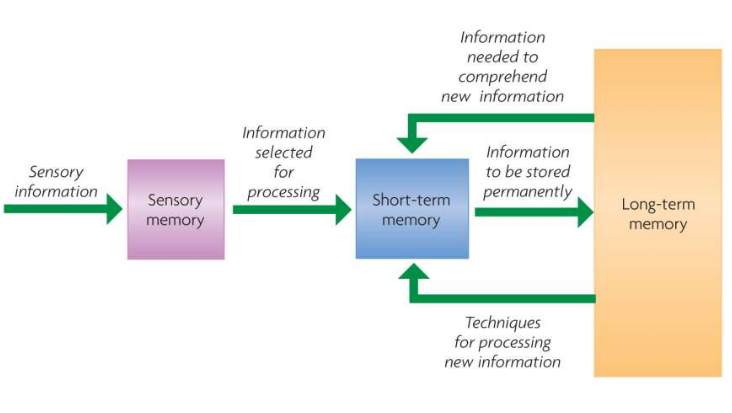
\includegraphics[width=0.8\textwidth]{../images/3-5-ipt}
	        \caption{The Three Fundamental Memory Systems}
	    \label{fig:3-5-ipt}
    \end{figure}
\subsubsection{Sensory Memory}
\begin{itemize}
\item A memory system that accurately but very briefly registers sensory information before the information
    fades or moves into short-term memory
    \item THe sensory register acts as a holding bin, retaining information accurately until we select information for \textbf{attention}.
    \item A snapshot of sensory information which lasts for less than \textbf{1 second}.
    \end{itemize}
    \begin{example}
Today, you probably heard a lot of conversations or faces. However, you probably don't remember them sense you didn't pay attention.
                                    \end{example}
\subsubsection{Short-Term Memory}
    \vocab{Short term memory} is the information you are currently using, this is why it is sometimes called \vocab{working memory}.\\

    However, it will disappear unless we undergo \vocab{repetitive rehearsal} to prevent the information from vanishing from the short-term memory.
    This could be by repeating it to yourself, either verbally or mentally.\\

What if the rehearsal is disrupted? Peterson \& Peterson tested this in Figure \ref{fig:3-5-pet} and found results shown in Figure \ref{fig:3-5-res}.
\begin{figure}[h!]
	    \centering
	    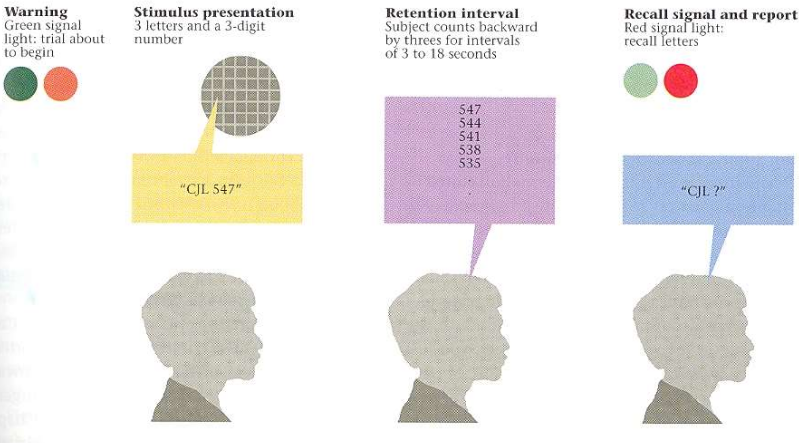
\includegraphics[width=0.8\textwidth]{../images/3-5-pet}
\caption{Peterson \& Peterson (1959) Disruption of Repetitive Recall}
	    \label{fig:3-5-pet}
    \end{figure}
\begin{figure}[h!]
	    \centering
	    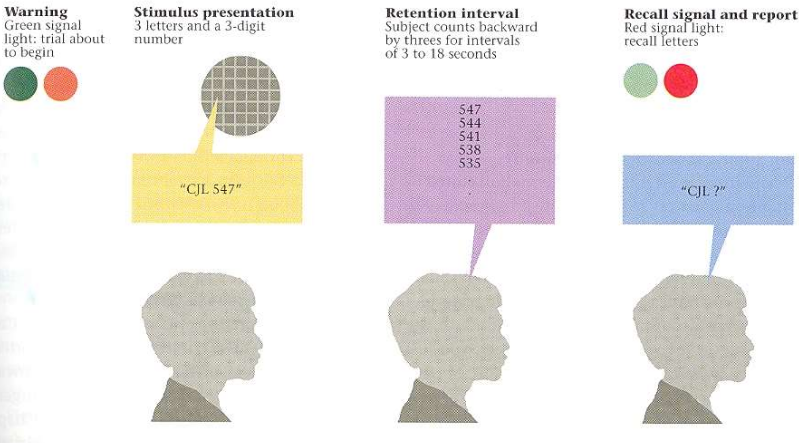
\includegraphics[width=0.8\textwidth]{../images/3-5-pet}
\caption{Results of Peterson \& Peterson (1959)}
	    \label{fig:3-5-res}
    \end{figure}
    \begin{remark}
The purpose of counting backwards by three is to prevent repetitive recall.
                                \end{remark}
    \begin{remark}
After about 15-25 seconds, memory begins to fade.
                                \end{remark}
Our short-term memory also has a capacity, which is seven $\pm$ 2 units.
    George Miller (1956) tested this by asking people to recall numbers in a random order.
  \subsubsection{Long-Term Memory}
\begin{itemize}
\item Long term memory is a seemingly unlimited capacity store that can hold information over lengthy periods of time.
    \item Information being maintained in STM through \vocab{elaborative rehearsal} is gradually absorbed into LTM.
    \begin{definition}
Elaborative rehearsal is when undergo deep semantic processing of a to-be-remembered item, such as jotting down notes or paraphrasing.
                                                \end{definition}

    \end{itemize}

\subsection{Age-Related Changes in Information Processing}
    As we age, our memory capacity increases, as shown in Figure \ref{fig:3-5-cap}.\\
\begin{figure}[h!]
	    \centering
	    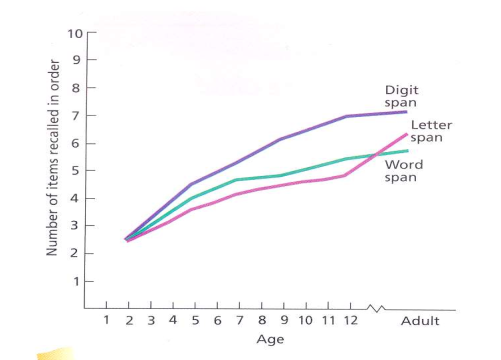
\includegraphics[width=0.8\textwidth]{../images/3-5-cap}
	                \caption{Increase of Memory Capacity as we Age}
	    \label{fig:3-5-cap}
    \end{figure}

    Besides capacity, we also have increased processing efficiency. One example of this is \vocab{automaticity}, where we can recall long-term memory without using short-term memory.
    \begin{example}
For example, what is $3\times 7$?
                                    \end{example}
    With automaticity, short-term memory is freed up for more complex tasks. \\

    Out attention also increases as we age. There are three aspects:

    \begin{description}
	    \item[Attention Span:] How long you can concentrate (e.g. in a lecture) without being distracted.
    \begin{example}
A two-year old can stay attentive for about 5 minutes. Most adults can stay attentive on one thing for around 20 min. However, we are better able to refocus on our task.
                                    \end{example}
    \item[Selective Attention:] Focus on one stimulus and tune out other.
    \begin{example}
Listening to a zoom class in a noisy environment.
                                    \end{example}
    \item[Divided Attention:] Pay attention to two or more sets of stimuli at the same time.
    \end{description}

There are a few different memory techniques:
    \begin{itemize}
\item Clustering: Grouping things together, start at around 2 years old.
\item Create a story (elaborative rehersal).
    \item Repetitive rehearsal: the process of repetitively verbalizing or thinking about information.
    \begin{example}
Children under 5 seldom use repetitive rehearsal, but children from 6-10 used it more.
                                    \end{example}

    \end{itemize}
\end{document}
